\section{Dataset exploration}
To gain an initial understanding of the dataset, we generated several insightful plots, which are presented below.
\subsection{Ingredient Frequency}
This plot represents the number of ingredients contained in the recipes of our dataset.
\begin{figure}[H]
    \centering
    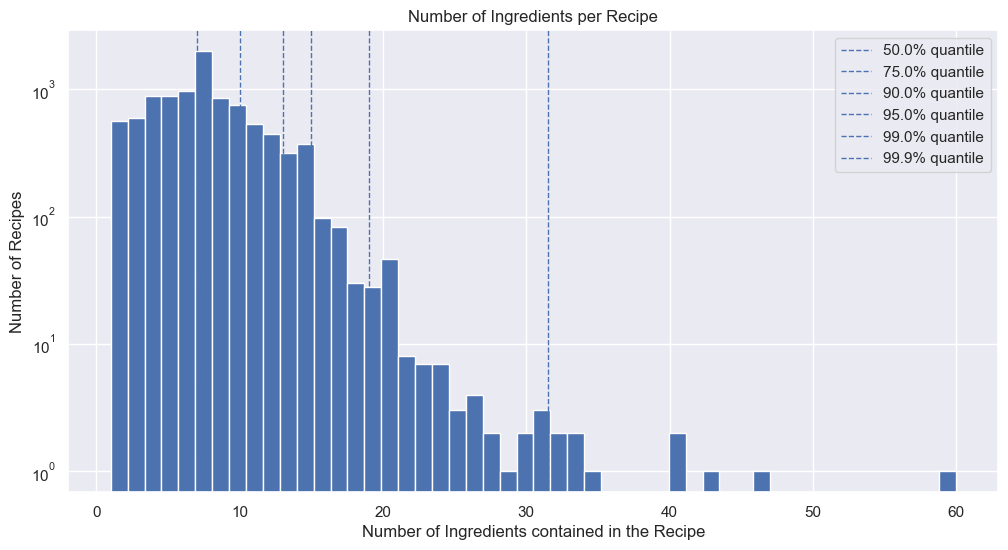
\includegraphics[width=\linewidth]{Report/ReportLatex/Images/Analisysplots/plot1.png}
    \caption{Plot 1}
    \label{fig:enter-label}
    \end{figure}
\subsection{Review Ratings Distribution}
This plot represents the distribution of the ratings in the dataset.
\begin{figure}[H]
    \centering
    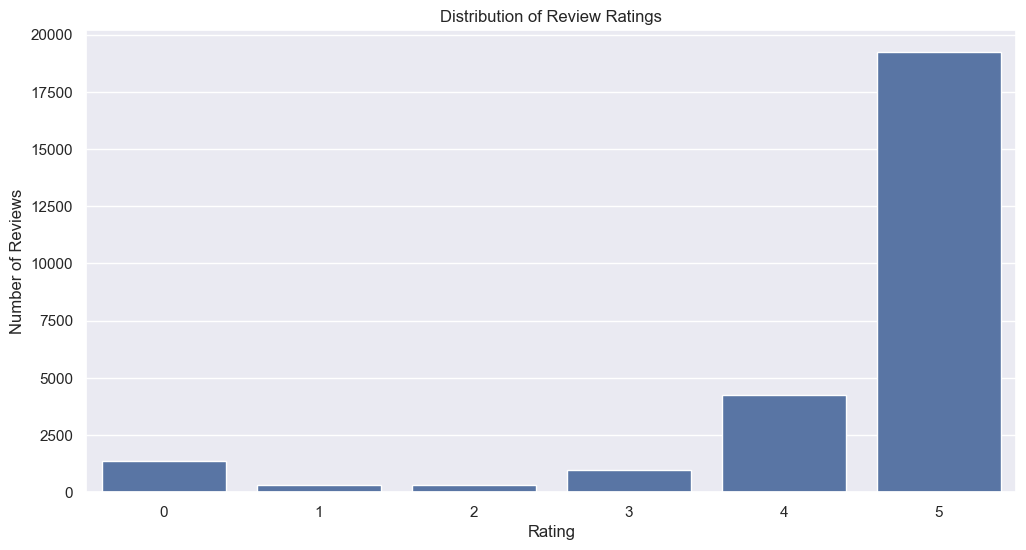
\includegraphics[width=\linewidth]{Report/ReportLatex/Images/Analisysplots/plot2.png}
    \caption{Plot 2}
    \label{fig:enter-label}
    \end{figure}
\subsection{Average rating per recipe distribution}
The Average Rating per Recipe Distribution plot provides an overview of how recipes are rated on average within the dataset.
\begin{figure}[H]
    \centering
    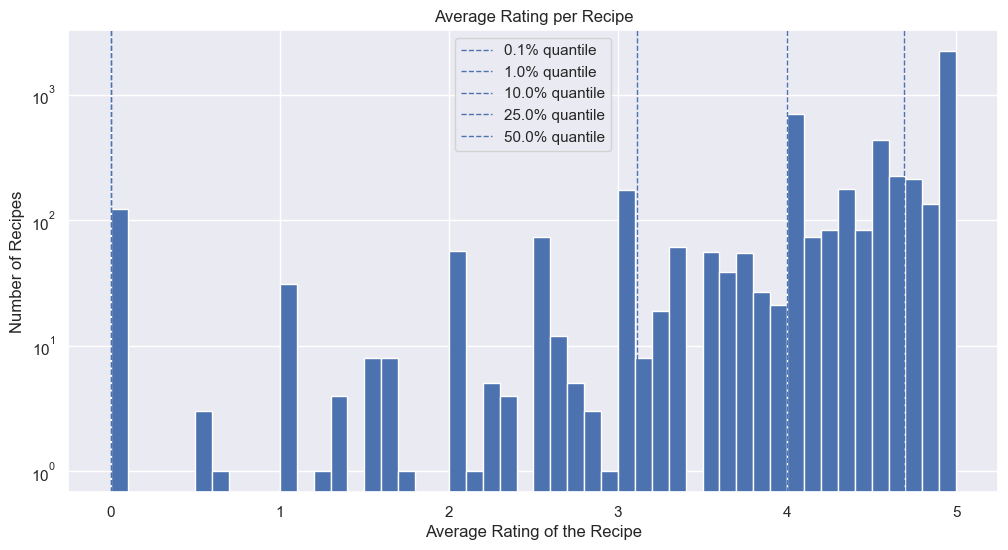
\includegraphics[width=\linewidth]{Report/ReportLatex/Images/Analisysplots/plot3.png}
    \caption{Plot 3}
    \label{fig:enter-label}
    \end{figure}
\subsection{Number of reviews per recipe distribution}
The Number of Reviews per Recipe Distribution plot shows how reviews are distributed across recipes, highlighting which recipes are highly reviewed and which receive fewer reviews.
\begin{figure}[H]
    \centering
    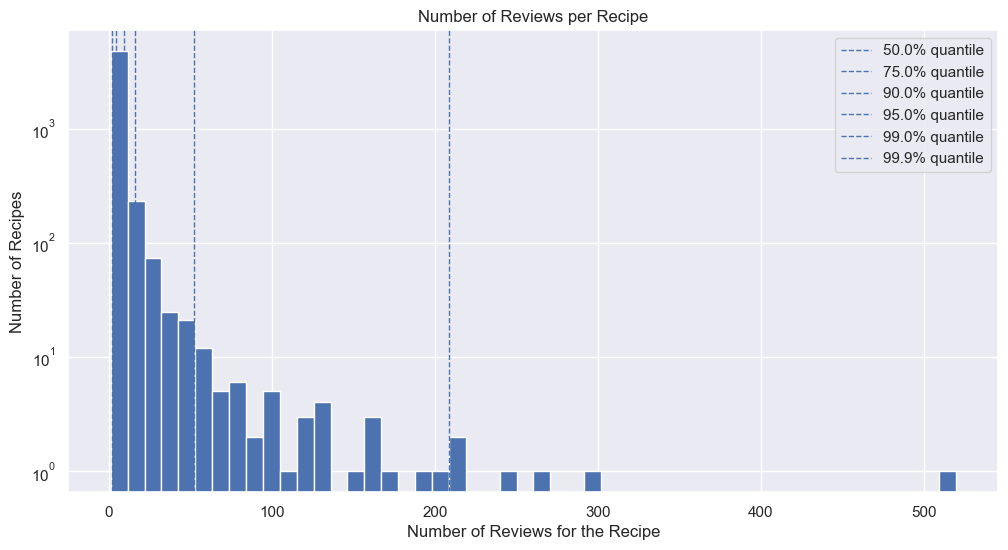
\includegraphics[width=\linewidth]{Report/ReportLatex/Images/Analisysplots/plot4.png}
    \caption{Plot 4}
    \label{fig:enter-label}
    \end{figure}
\section{Neo4j}
In the following pages, it is reported the model and the code used to load the dataset into a Neo4J instance. 
Six different type of nodes have been identified:
\begin{itemize}
    \item \textbf{Recipe}: It represents a recipe of the dataset and it has various attributes
          \begin{itemize}
              \item RecipeId: this attribute is an integer that uniquely identifies each recipe. To ensure its uniqueness, a constraint is enforced on this attribute.
              \item Name: attribute representing the name of a recipe.
              \item Calories: it is a float value representing the calorie content of a recipe. During data loading, tofloat() function is used to ensure that this value is correctly interpreted as a numeric data type rather than a string.
              \item CookTime: this value represents the cooking time of the recipe, formatted according to ISO 8601. Since Neo4j supports this format,  the duration() function is used to handle this attribute as a time value.
              \item PrepTime: this value represents the preparation time of the recipe, formatted in accordance with ISO 8601. Here too, the duration() function is used to handle this attribute as a time value.
              \item TotalTime: this value is defined as the sum of the preparation and cooking times, representing the total time required for the recipe. The duration() function is also used to handle this attribute.
              \item FatContent: this float value represents the fat content of the recipe. The tofloat() function is applied to ensure it is processed as a numeric value.
              \item ProteinContent: this float value represents the protein content of the recipe. The tofloat() function is used to ensure it is processed as a numeric value.
              \item CarbohydrateContent: this float value represents the carbohydrate content of the recipe. The tofloat() function is applied to ensure it is processed as a numeric value.
              \item RecipeServings: this number represents the servings for the recipe. The tointeger() function is used to ensure it is processed as a numeric value.
          \end{itemize}
    \item \textbf{Ingredient}: Ingredients are connected to Recipe via the CONTAINS relationship, and their sole attribute is name, which is used to enforce uniqueness of the ingredient through a constraint. In the dataset, ingredients were initially represented as a list for each recipe. During data loading, the data are first cleaned by removing unnecessary elements such as commas and parentheses. Then, the UNWIND operation is used to create individual ingredient nodes. Recipes with missing ingredients, or ingredients labeled as "character(0," are excluded by applying a WHERE clause.
    \item \textbf{RecipeCategory}: this node represents the category to which the recipe belongs. The coalesce() function is used to assign the value "Unknown" as the category in case the value was missing. Additionally,the name attribute is used to enforce the uniqueness of the category through a constraint. The node recipe is connected to the category using the relationship BELONGS\_TO.
    \item \textbf{Keyword}: a keyword is a word that describes the recipe. The uniqueness of each keyword is ensured by applying a constraint to its name attribute. In the dataset, keywords were represented as a list for each recipe. After cleaning the data, the UNWIND operation is used to create individual nodes for each keyword. Recipes are connected to keywords via the DESCRIBED\_BY relationship.
    \item \textbf{Review}: this node represents a review written for a recipe. It is identified by a unique integer id, for which a constraint is applied to ensure its uniqueness. The review also contains an integer rating value. The toInteger() function is used for it to treat it as numeric values. The review is connected to both the Recipe and User nodes via the FOR and WROTE relationships, respectively.
    \item \textbf{User}: this node represents users in the dataset, whether they created a recipe or wrote a review. Each user is identified by a unique id, for which a constraint is applied to ensure its uniqueness. The node also contains the name attribute. Users are connected to reviews via the WROTE relationship and to recipes via the CREATED\_BY relationship.
\end{itemize}
\subsection{Data Model}
\begin{figure}[H]
    \centering
    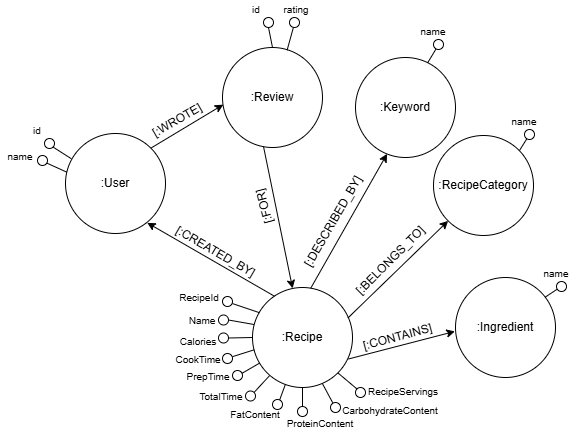
\includegraphics[width=\linewidth]{Report/ReportLatex/Images/Neo4J/graph.png}
    \caption{Data Model}
    \label{fig:enter-label}
    \end{figure}
\subsection{Constraints}
The following constraints check that every node created is unique.
\begin{CypherQuery}
MATCH
CREATE CONSTRAINT FOR (recipe:Recipe) REQUIRE recipe.id IS UNIQUE;

CREATE CONSTRAINT FOR (ingredient:Ingredient) 
REQUIRE ingredient.name IS UNIQUE;

CREATE CONSTRAINT FOR (keyword:Keyword) REQUIRE keyword.name IS UNIQUE;

CREATE CONSTRAINT FOR (recipeCategory:RecipeCategory)
REQUIRE recipeCategory.name IS UNIQUE;

CREATE CONSTRAINT FOR (user:User) REQUIRE user.id IS UNIQUE;

CREATE CONSTRAINT FOR (review:Review) REQUIRE review.id IS UNIQUE;

\end{CypherQuery}
\subsection{Data loading}
The following is the Cypher code it is used to load the data. Both CSV files were loaded and merged, ensuring that no duplicates were created and that each relationship correctly connected to the appropriate nodes.
\begin{CypherQuery}
-
LOAD CSV WITH HEADERS FROM "file:/recipes(10000).csv" AS row
WITH row
WHERE row.RecipeId IS NOT null
MERGE (r:Recipe { id: row.RecipeId })
ON CREATE SET r.Name = row.Name, r.Calories = tofloat(row.Calories), r.RecipeServings = tointeger(row.RecipeServings), r.CookTime = duration(row.CookTime), r.PrepTime = duration(row.PrepTime), r.TotalTime = duration(row.TotalTime), r.FatContent = tofloat(row.FatContent), r.CarbohydrateContent = tofloat(row.CarbohydrateContent), r.ProteinContent = tofloat(row.ProteinContent)

WITH r, row, trim(replace(row.Keywords, "c(", "")) AS cleaned_keywords
WITH r, row, trim(replace(cleaned_keywords, ")", "")) AS final_keywords
WITH r, row, split(replace(final_keywords, "'", ""), ", ") AS keywords
UNWIND keywords AS keyword
MERGE (k:Keyword { name: keyword })
MERGE (r)-[: DESCRIBED_BY ]->(k)

WITH r, row, trim(replace(row.RecipeIngredientParts, "c(", "")) AS cleaned_ingredients
WITH r, row, trim(replace(cleaned_ingredients, ")", "")) AS final_ingredients
WITH r, row, split(replace(final_ingredients, "'", ""), ", ") AS ingredients
UNWIND ingredients AS ingredient
WITH r, row, ingredient
WHERE ingredient <> "character(0"
MERGE (i:Ingredient {name: ingredient})
MERGE (r)-[: CONTAINS ]->(i)

MERGE (rc:RecipeCategory { name: coalesce(row.RecipeCategory, 'Unknown') })
MERGE (r)-[: BELONGS_TO ]->(rc)

WITH r, row
MERGE (u:User { id: row.AuthorId })
// Ensure the name is set only on creation
ON CREATE SET u.name = row.AuthorName 
MERGE (r)-[: CREATED_BY ]->(u)

LOAD CSV WITH HEADERS FROM "file:/reviews(10000).csv" AS reviewRow
WITH reviewRow
WHERE reviewRow.RecipeId IS NOT null
MERGE (reviewer:User { id: reviewRow.AuthorId })
ON CREATE SET reviewer.name = reviewRow.AuthorName 
// Ensure name is set only on creation

WITH reviewRow, reviewer
MERGE (review:Review { id: reviewRow.ReviewId, rating: tointeger(reviewRow.Rating) })

// Match the Recipe with the corresponding RecipeId from the reviews.csv
WITH reviewRow, reviewer, review
MATCH (recipe:Recipe { id: reviewRow.RecipeId })
WITH recipe, reviewRow, reviewer, review
MERGE (reviewer)-[:WROTE]->(review)
MERGE (review)-[:FOR]->(recipe)
\end{CypherQuery}
\section{Elasticsearch}
\subsection{Mapping}

The mapping for the index was defined statically, avoiding the use of dynamic mapping to prevent potential issues. This mapping covers every attribute in our dataset and gives a structure for the documents stored in the index.

Fields such as RecipeId, AuthorId, and ReviewId were set as type keyword, as they contain structured, consistent content that does not require analysis or tokenization for search purposes. 

For fields containing textual content, such as names, instructions, and reviews, the text field type is used and the standard analyzer is applied. This allows Elasticsearch to perform full-text searches and relevance-based querying.

Numerical fields, like the ones for quantities and times, were mapped as either float or integer, depending on the specific requirements of the data. 

Dates in the dataset were defined as date fields with the "strict\_date\_time" format, which matches the dataset’s date representation. The strict\_date\_time format follows the pattern yyyy-MM-dd"T"HH:mm:ss.SSSZ, for example, 2023-12-17T15:30:00.000Z.

In our mapping, certain fields are configured with "index": false. This setting ensures that these fields are not searchable or usable in filtering operations.

Because the dataset includes a varying number of reviews for each recipe, structured in an array, nested fields were used. Nested fields in Elasticsearch are a special type of field that allows arrays of objects to be indexed and queried as independent units. Each review is a structured object with attributes such as ReviewId, Rating, AuthorName, and the review text itself.

\begin{lstlisting}[language=Elasticsearch]
PUT /recipesandreviews
{
  "mappings": {
    "properties": {
      "RecipeId": {
        "type": "keyword"
      },
      "Name": {
        "type": "text",
        "analyzer": "standard"
      },
      "AuthorId": {
        "type": "keyword"
      },
      "AuthorName": {
        "type": "text",
        "analyzer": "standard"
      },
      "CookTime": {
        "type": "integer"
      },
      "PrepTime": {
        "type": "integer"
      },
      "TotalTime": {
        "type": "integer"
      },
      "DatePublished": {
        "type": "date",
        "format": "strict_date_time"
      },
      "Description": {
        "type": "text",
        "analyzer": "standard"
      },
      "Images": {
        "type": "text",
        "index": false
      },
      "RecipeCategory": {
        "type": "text",
        "analyzer": "standard"
      },
      "Keywords": {
        "type": "text",
        "analyzer": "standard"
      },
      "RecipeIngredientQuantities": {
        "type": "text",
        "analyzer": "standard"
      },
      "RecipeIngredientParts": {
        "type": "text",
        "analyzer": "standard"
      },
      "AggregatedRating": {
        "type": "float"
      },
      "ReviewCount": {
        "type": "integer"
      },
      "Calories": {
        "type": "float"
      },
      "FatContent": {
        "type": "float"
      },
      "SaturatedFatContent": {
        "type": "float"
      },
      "CholesterolContent": {
        "type": "float"
      },
      "SodiumContent": {
        "type": "float"
      },
      "CarbohydrateContent": {
        "type": "float"
      },
      "FiberContent": {
        "type": "float"
      },
      "SugarContent": {
        "type": "float"
      },
      "ProteinContent": {
        "type": "float"
      },
      "RecipeServings": {
        "type": "float"
      },
      "RecipeYield": {
        "type": "text",
        "index": false
      },
      "RecipeInstructions": {
        "type": "text",
        "analyzer": "standard"
      },
      "Reviews": {
        "type": "nested", 
        "properties": {
          "ReviewId": {
            "type": "keyword"
          },
          "RecipeId": {
            "type": "keyword"
          },
          "AuthorId": {
            "type": "keyword"
          },
          "AuthorName": {
            "type": "text",
            "analyzer": "standard"
          },
          "Rating": {
            "type": "float"
          },
          "Review": {
            "type": "text",
            "analyzer": "standard"
          },
          "DateSubmitted": {
            "type": "date",
            "format": "strict_date_time"
          },
          "DateModified": {
            "type": "date",
            "format": "strict_date_time"
          }
        }
      }
    }
  }
}
\end{lstlisting}